% !TEX root =  master.tex 
\chapter{SonarQube -- Manuel Techert}


\section{Definition von SonarQube}

Die von uns eingesetzte Plattform SonarQube wird hier kurz erklärt.

Die Plattform SonarQube wird in der offiziellen Dokumentation von Ann Campbell folgendermaßen definiert:

\enquote{The SonarQube® platform is an open source quality management platform, dedicated to continuously analyzing and measuring the technical quality of source code, from project portfolio down to the method level, and tracking the introduction of new Bugs, Vulnerabilities, and Code Smells in the Leak Period} \autocite{DefinitionSonarQubeDoc}.

Diese Definition deckt sich mit dem Leitsatz der offiziellen Homepage von SonarQube. Demnach soll SonarQube  die Qualität eines Produktes laufend anhand von Analysen und Kennzahlen protokollieren und etwaige Fehler verfolgbar machen \autocite[Vgl.][]{StartSeiteSonarQube}.


\section{Aufbau und grundlegende technische Voraussetzungen}

\subsection{Die drei Komponenten von SonarQube}

SonarQube ist kein eigenständiges Werkzeug. Es ist eine Plattform, die sich aus drei wesentlichen Komponenten ergibt. 
So besteht diese aus einem SonarQube-Server, der unter anderem für die Verarbeitung und Aufbereitung der Analysen zuständig ist, dessen Ergebnisse sich gespeichert in der zweiten Komponente, der Datenbank, wiederfinden. Zuletzt existiert noch der Scanner, welcher die Analysen übernimmt.


\begin{minipage}{\linewidth}
	\centering
	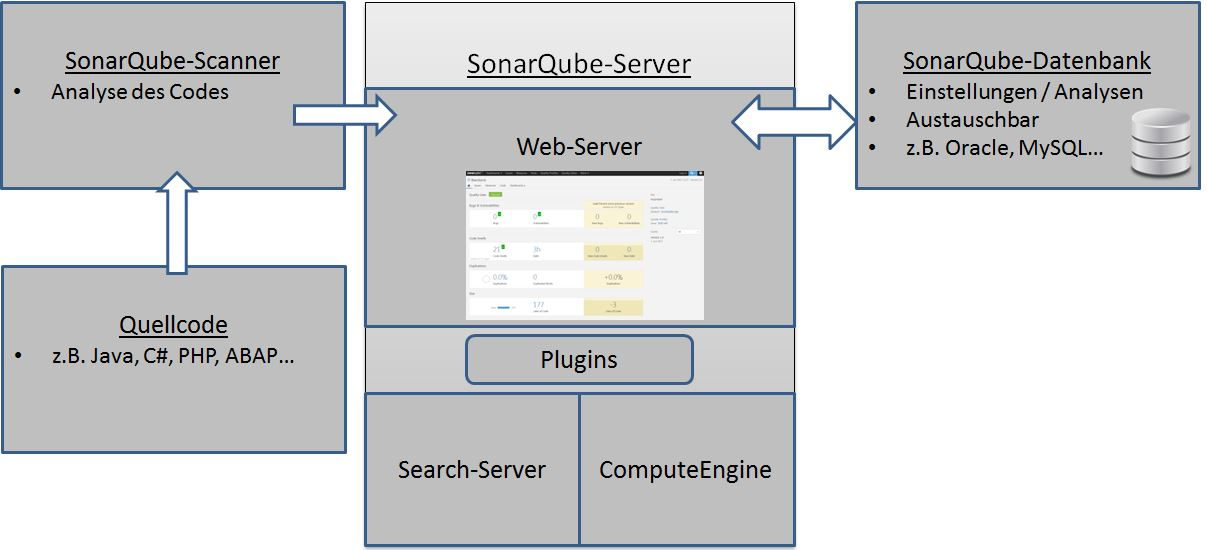
\includegraphics[scale=0.45]{img/SonarAufbau.jpg}
	\captionof{figure}{\label{abb:sonaraufbau}Der Aufbau der Komponenten von SonarQube}
	\vspace{2em}
\end{minipage}

\subsubsection{Der SonarQube-Server}

Der SonarQube-Server, der die Schnittstelle zwischen dem Scanner und der Datenbank darstellt, besteht aus einem \glqq ComputeEngine-Server\grqq{}, dem \glqq Search-Server\grqq{} und zuletzt dem \glqq Web-Server\grqq{} \autocite[Vgl.][]{dotnetpro}.

Wird eine Analyse mithilfe des Scanners durchgeführt, verarbeitet der ComputeEngine-Server diese, um sie im Anschluss in der Datenbank abspeichern zu können.

Sind nun Analysen in der Datenbank hinterlegt, sucht der Search-Server gezielt nach diesen, um sie weiter auf den Web-Server zu reichen.

Im Interface des Web-Servers können schließlich die Ergebnisse der Analysen begutachtet werden. Hier finden sich neben zahlreichen Möglichkeiten, die Ergebnisse zu filtern und zu betrachten, auch diverse Einstellungsmöglichkeiten für SonarQube selbst.

\subsubsection{Die Datenbank}

In der Datenbank werden alle vorgenommenen Einstellungen und Analysen abgespeichert. Eine Eigene ist bei der Installation von SonarQube bereits integriert. Diese ist aber nicht bindend, es können auch Datenbanken wie Microsoft SQL Server, MySQL, Oracle oder PostgreSQL genutzt werden \autocite[Vgl.][]{SonarRequirements}. Da die Menge an analysierten Daten schnell unübersichtlich groß wird, sollte man bei einer ernsthaften Verwendung von SonarQube in jedem Fall die ursprüngliche Datenbank ersetzen.

\subsubsection{Der Scanner}

Der Scanner bildet die Grundlage für Analysen und ist, neben einer lokalen Variante, in verschiedenen Versionen für die unterschiedlichsten Build-Tools verfügbar \autocite[Vgl.][]{VerschScanner}. Diese Tools werden im Softwareentwicklungsprozess oft genutzt, um den Prozess vom Programmieren zum ausführbaren Programm vereinfacht zu verwalten \autocite[Vgl.][]{BuildTools}. Ein Beispiel für solch ein Tool ist Apache Maven, welches auf der offiziellen Seite als \enquote{[...] software project management and comprehension tool.} beschrieben wird \autocite{Maven}.

Ganz gleich in welcher Version, bedient der Scanner sich, um seine Analyse durchführen zu können,  dreierlei Werkzeuge:  \glqq FindBugs\grqq{}, \glqq PMD\grqq{} und \glqq CheckStyle\grqq{} \autocite[Vgl.][]{FindBugsPMDCheckStyle}. Diese Werkzeuge besitzen eigene Metriken, die gegebenen Quelltext oder kompilierten Bytecode hinsichtlich verschiedener Kriterien durchsuchen. 

Der Begriff \enquote{Metrik} ist dabei durch einen IEEE-Standard folgendermaßen normiert:

\enquote{A function whose inputs are software data and whose output is a single numerical value that can be interpreted as the degree to which software possesses a given attribute that affects its quality.}\autocite{IEEE1061-1998}.

Demnach ist eine Metrik eine Funktion, welche aus einem Eingabestrom Ausgabewerte erzeugt, die untereinander vergleichbar sind. Diese Werte sind in der Softwaremetrik Zahlen, deren Höhe Auskunft über die Qualität eines Teils einer Software geben.

Alle Metriken sind in sogenannten Regeln umgesetzt, deren Verstöße, \enquote{Issues} genannt, vermerkt werden.

FindBugs durchsucht den vom Java-Compiler übersetzten Bytecode auf strenge Programmierfehler, wie etwa nicht mögliche Typumwandlungen \autocite[Vgl.][]{FindBugs}. Fehler, die also aufgrund fehlender Kenntnisse oder Flüchtigkeit entstehen, werden von FindBugs entdeckt.

Das nächste Werkzeug, PMD, befasst sich weniger mit Fehlern, sondern eher mit einer Steigerung der Effizienz \autocite[Vgl.][]{PMD}. PMD erkennt somit alles, was optimiert zu einer Leistungssteigerung führt. Beispiele hierfür sind etwa leere Code-Blöcke, die keinen Inhalt haben und damit obsolet sind. Noch ein Beispiel stellen Variablen dar, die zwar initialisiert, aber nie benutzt werden.  Dieses Werkzeug arbeitet, anders als FindBugs nicht auf Bytecode-, sondern auf Quelltextebene.

Zuletzt bedient sich der Scanner noch am Werkzeug CheckStyle. Dieses arbeitet, wie PMD, auf Quelltextebene und prüft die Einhaltung bestimmter Programmier-Konventionen. So sind die hier erkannten \enquote{Fehler} lediglich Vorschläge, die zu einem besseren Stil beitragen und das Programm beispielsweise übersichtlicher machen \autocite[Vgl.][]{CheckStyle}.

Nach dieser Einteilung des Fehlertyps werden Verstöße noch in ihrer Schwere beurteilt. Je nachdem, wie gravierend ein Verstoß wiegt, wird dieser von der Schwere hin absteigend zum Beispiel als \enquote{Blocker} oder \enquote{Critical}, \enquote{Major} oder \enquote{Minor} deklariert \autocite[Vgl.][]{MetricDefinitions}. Auch eine Einstufung als \enquote{Info} ist möglich. Ein Verstoß wird also einmal in seiner Art und darüber hinaus in der Schwere beurteilt.
Alle Stellen im Code, wo eine Optimierung notwendig oder möglich ist, werden durch den Scanner markiert und im Web-Server aufbereitet angezeigt. Die Erkennung läuft bei allen Werkzeugen gleichermaßen ab. Individuell einstellbare Regeln jedes Werkzeugs werden auf ihre Erfüllung hin abgeprüft und Verstöße entsprechend aufgezeigt. Wie in der Einleitung bereits erwähnt, werden alle Regeln bezüglich ihrer Kategorie noch in eine der Sparten Bugs, Code Smells oder Vulnerabilities eingeordnet.


\section{Inbetriebnahme von SonarQube - Überblick}
%und richtige Interpretation der Daten}

SonarQube wird von uns über eine manuelle Installation wie folgt installiert:

Zunächst erfolgt ein Download des SonarQube-Server und eine anschließende Installation. Nach dessen Start kann der Scanner hinzugefügt werden, der nun Projekte analysieren kann. Dies erfolgt über das Terminal in in macOS. Analysierte Projekte werden bei einer nicht an das Internet gebundenen Installation, wie in unserem Fall, unter einer lokalen Webkomponente verfügbar gemacht \autocite[Vgl.][]{GetStarted}.

Ist SonarQube also vollständig installiert, der Server gestartet und wurde bereits eine Analyse durchgeführt, so kann man nun die Ergebnisse in der Webkomponente unter der angegebenen Adresse einsehen. Diese ist im Terminal nach Start des Servers zu sehen. Auf der Startseite des Web-Servers kann nun das untersuchte Projekt angewählt werden (siehe Abbildung 3.2). Die Reiter am oberen Rand, wie zum Beispiel \enquote{Dashboards}, \enquote{Issues} oder \enquote{Quality Gates} stellen allgemeine Optionen der Plattform dar.



\begin{minipage}{\linewidth}
	\centering
	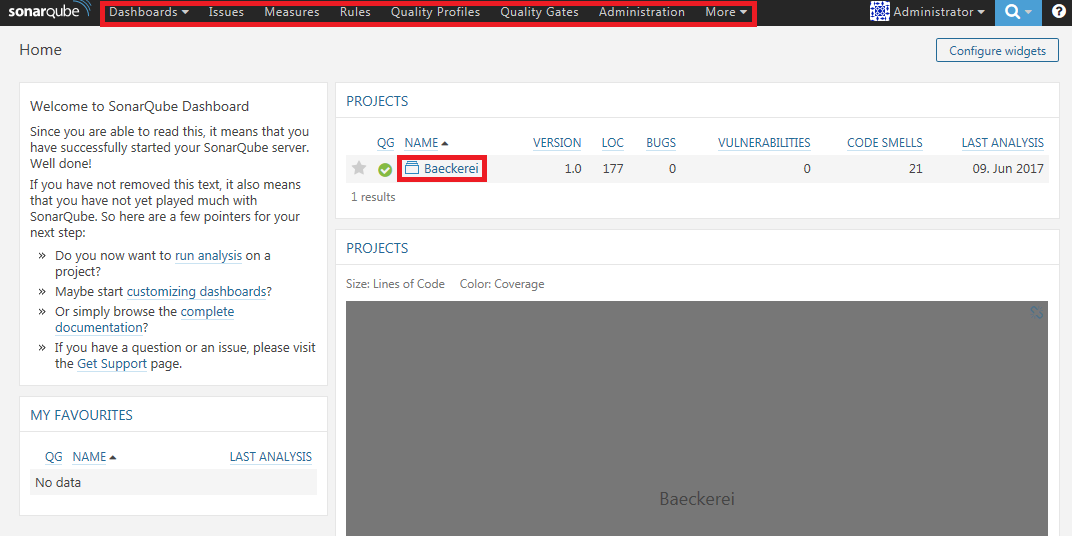
\includegraphics[scale=0.55]{img/StartSeiteSonar.PNG}
	\captionof{figure}{\label{abb:startseitesonar}Die Startseite des Web-Servers}
	\vspace{2em}
\end{minipage}

Sobald ein Projekt ausgewählt wurde, findet sich darunter ein sekundärer Reiter, der explizit das Projekt betrachtet (siehe Abbildung 3.3). Nun befindet man sich auf dem Dashboard eines Projektes. Neben dem erwähnten sekundären Reiter, ist hier eine gute Übersicht über die Merkmale des Projekts gegeben. Unter der Anzahl der \enquote{Bugs und Vulnerabilities} oder den \enquote{Code Smells}, findet man auch Werte für Duplikationen oder die Größe des untersuchten Codes. Auf der rechten Seite sind auch das zugewiesene Quality-Profile oder Quality-Gate aufgeführt.

Mit einem Klick auf \enquote{Issues} kann man alle Regelverstöße einsehen, die das Projekt verursacht hat. Die Sparte \enquote{Measures} präsentiert weitere Qualitätsmerkmale des Projektes, unter anderem \enquote{Reliability}, \enquote{Security} oder \enquote{Maintainability}. Unter \enquote{Code} findet man die Dateistruktur des Projektes, also die Aufteilung in die verschiedenen Packages und Klassen. Ist man mit dem Standard-Dashboard nicht zufrieden, gibt es die Option unter \enquote{Dashboards} seine eigene Übersicht aus zahlreichen Komponenten zusammenzubauen. Der letzte Punkt im Projektreiter, \enquote{Administration} ist nur sichtbar, wenn man als Administrator angemeldet ist und bietet diverse Verwaltungsmöglichkeiten für Speicherzeiträume der Datenbank, Quality-Profiles oder Quality-Gates. Die Rechteverwaltung findet man hier ebenso.



\begin{minipage}{\linewidth}
	\centering
	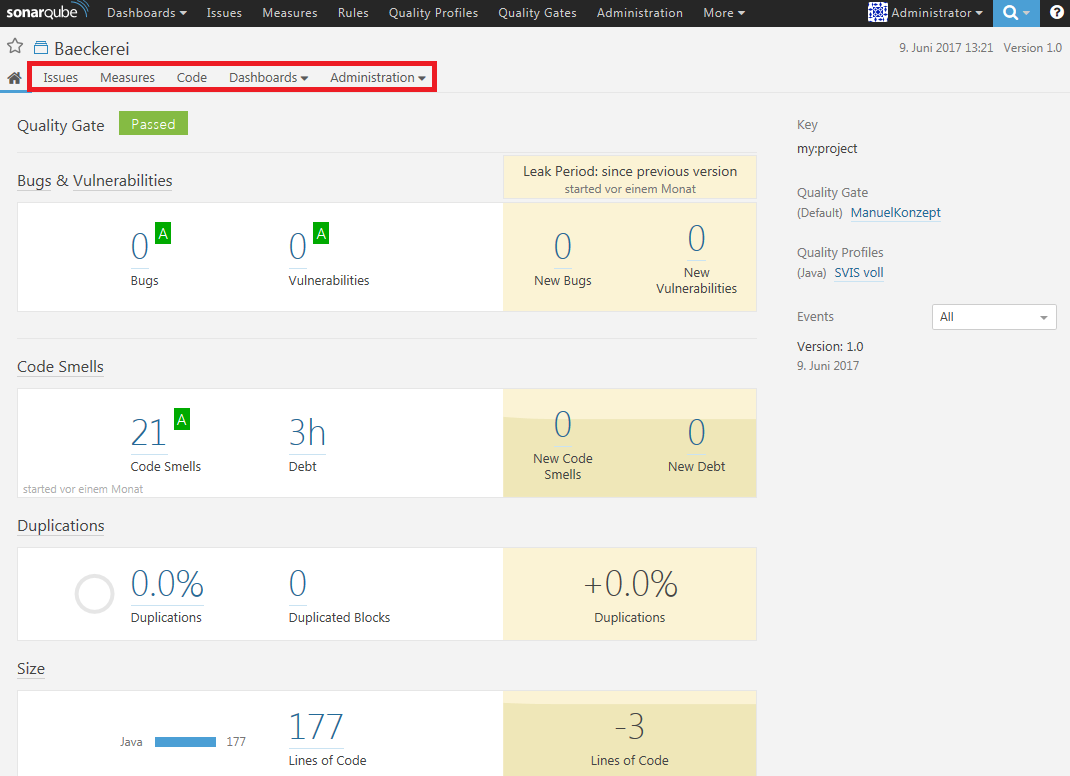
\includegraphics[scale=0.5]{img/StartSeiteSonarNachProjekt.PNG}
	\captionof{figure}{\label{abb:startseitesonarnachprojekt}Das Dashboard}
	\vspace{2em}
\end{minipage}


%Analysen durchführen, durch Filtern ersichtlich machen.
%Fehler verfolgen, evtl. durch Assignments auf einzelne User herunterbrechen.
%Fehler korrigieren, Regeln verstehen
%Fehler kritisch hinterfragen

\subsection{Quality-Profiles erstellen und verwalten}

Die die Analyse des Scanners bestimmenden Regeln können in SonarQube angepasst werden. In einem sogenannten Quality-Profile kann man festlegen, welche Regeln man aus dem Standard-Regelsatz von SonarQube, \enquote{TheSonarWay}, übernehmen möchte \autocite[Vgl.][]{QualityProfile}. So kann man individuell wichtige Regeln aktivieren und nicht benötigte oder störende abschalten.

Die Regeln selbst sind wieder in die drei Kategorien Bugs, Vulnerabilities und Code Smells unterteilt. Bei einem Verstoß gegen eine Regel, wird dieser entsprechend mit seiner zugehörigen Kategorie angezeigt. Wird also ein Verstoß gegen eine Regel aus dem Bereich \enquote{Bugs} erkannt, wird im Web-Server der Verstoß ebenso als Bug deklariert. Bei einigen Regeln kann man die darin enthaltenen Kriterien mit verschiedenen Parametern auf die Empfindlichkeit anpassen.
Jedem Projekt, also jeder Ansammlung von Klassen aus einer beliebig unterstützten Programmiersprache kann zu jeder Zeit genau ein Quality-Profile zur Nutzung zugewiesen werden, nach dessen Regeln es untersucht wird. Zusätzlich ist ein Standard-Quality-Profile festgelegt, das auch dann greift, wenn die Verbindung zum Server fehlt und damit das zu nutzende Profile nicht geladen werden kann \autocite[Vgl.][]{QualityProfile}. Beim Erstellen neuer Quality-Profiles ist es auch möglich, Regeln von anderen Profilen zu erben, um sich so das aufwendige Einfügen gleicher Regeln zu ersparen. Ebenso können Quality-Profiles heruntergeladen und wiederhergestellt werden. Dies geschieht über die Optionen \enquote{Restore} und \enquote{Backup} unter der Kategorie \enquote{Quality-Profiles}. Gespeichert werden die Profile im .xml-Format. Somit lassen sich präferierte Regeln auch über mehrere Versionen hinweg sichern und wiederherstellen \autocite[Vgl.][]{QualityProfile}.
Wir haben aus dem großen Regelsatz die für uns wichtigsten Regeln ausgewählt und diese in einem Quality-Profile namens \enquote{fallstudie} gesammelt und danach aktiviert.

\subsection{Quality-Gate anpassen}

Um nun die Qualität der eigenen Software besser verfolgen zu können, kann man \enquote{Quality-Gates} auf dem SonarQube-Server einrichten, die als metaphorisches Prüftor dienen, welches die Software passieren muss \autocite[Vgl.][]{QualityGate}. Die Anwendung passiert dieses Tor nur dann, wenn vorher gesetzte Anforderungen erfüllt sind. Ist dies nicht der Fall, kann die Software nicht passieren.

Unter anderem kann bei der Einrichtung eines solchen Gates festgelegt werden, wie schwer verschiedene Arten von Fehlern wiegen oder wie viele Fälle eine \enquote{case} -Anweisung in der Programmiersprache Java höchstens haben darf. Diese Anforderungen sind alle vollständig frei setzbar und dienen daher dazu, die eigenen Qualitätsanforderungen an die Software besser umsetzen zu können. Noch dazu wird unterschieden, ob ein gewisses Kriterium zu jeder Zeit erfüllt werden muss oder nur über einen längeren Zeitraum gegeben sein muss \autocite[Vgl.][]{QualityGate}. 
Als kleines Beispiel kann eingestellt werden, dass die Software zu jeder Zeit nur fünf Bugs haben darf. Führt man nun eine Analyse durch und betrachtet die Ergebnisse, wird zugleich ausgegeben, ob die Software den Anforderungen des Quality-Gates gerecht geworden ist und somit passieren kann oder ob hier noch nachgearbeitet werden muss. Bei vier Bugs zu einem beliebigen Zeitpunkt würde das Gate passiert werden, ab sechs nicht mehr.

Generell ist immer eine Bedingung in Kombination mit einem Operator, wie z.B. \enquote{größer}, \enquote{kleiner} oder \enquote{gleich} wählbar. Dazu kommen noch zwei Richtwerte, die gesetzt werden müssen, um festzulegen, ab welchem Wert, in Verbindung mit dem Operator, ein Error oder eine Warnung erzeugt wird. Analog zu den Quality-Profiles können die Einstellungen zum Quality-Gate im Webinterface vorgenommen werden. Auch das als Standard zu nutzende Quality-Gate muss festgelegt werden, da ansonsten wieder auf das von der Installation mitgebrachte Quality-Gate zugegriffen wird.

Da uns primär das Finden von Fehlerquellen wichtig war, haben wir die Einstellungen des Quality-Gates zunächst auf den Standard-Einstellungen gelassen, die bestimmten, das keine neuen, schweren Issues hinzukommen dürfen. So haben wir laufend versucht, von vorneherein Fehlerquellen gar nicht erst entstehen zu lassen.


\begin{minipage}{\linewidth}
	\centering
	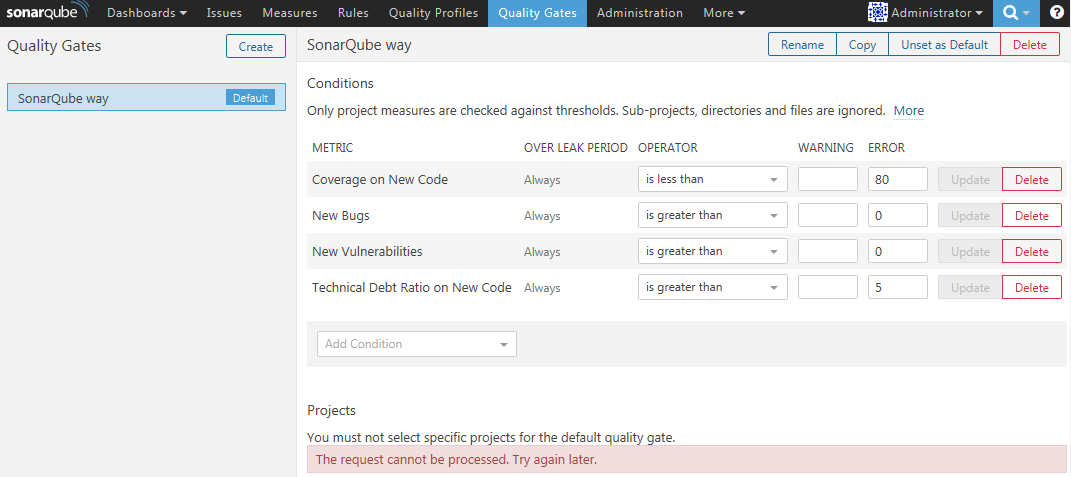
\includegraphics[scale=0.55]{img/QualityGate.PNG}
	\captionof{figure}{\label{abb:qualitygate}Beispielkonfiguration eines Quality-Gates}
	\vspace{2em}
\end{minipage}

